\documentclass[twocolumn]{IEEEtran}
\usepackage{graphicx}
\usepackage[utf8x]{inputenc}
\usepackage{times}
\usepackage{amssymb,amsfonts}
\usepackage[tbtags]{amsmath}
\usepackage{cite}
\usepackage{pict2e}
\usepackage{float}
\usepackage{lscape}
\usepackage[all]{xy}
\usepackage{graphics,graphicx,color,colortbl}
\usepackage{times}
\usepackage{subfigure}
\usepackage{wrapfig}
\usepackage{multicol}
\usepackage{cite}
\usepackage{url}
\usepackage[tbtags]{amsmath}
\usepackage{amsmath,amssymb,amsfonts,amsbsy}
\usepackage{listings}
\usepackage{bm}
\usepackage{algorithm}
\usepackage{algorithmic}
\usepackage[centerlast, small]{caption}
\usepackage[colorlinks=true, citecolor=blue, linkcolor=blue, urlcolor=blue, breaklinks=true]{hyperref}
\hyphenation{ele-men-tos he-rra-mi-en-ta cons-tru-yen trans-fe-ren-ci-a pro-pu-es-tas si-mu-lar vi-sua-li-za-cion}

\begin{document}
\title{Introducción al uso del procesador LatticeMico32}
\author{José Alejandro Logreira Ávila Código: $261722$\\
	David Ricardo Martínez Hernández Código: $261931$\\
	Edwin Fernando Pineda Vargas Código: $262100$}
\maketitle
\markboth{Universidad Nacional de Colombia}{}
\floatname{algorithm}{Algoritmo}
\begin{keywords}
 Bits, Datapath, Makefile, Memoria, MIPS, Pipeline, Síntesis, Variables.
\end{keywords}

\begin{abstract}
 Se realizo la instalación de todas las herramientas necesarias en el sistema operativo Linux, distribución Ubuntu, basándonos en la pagina principal de Linux En Caja para la instalación de dichas herramientas. Realizando todas las actividades propuestas en la guía de laboratorio, obteniendo algunos de los resultados de manera eficiente y completa, ya que existieron muchas dificultades al momento de instalar y utilizar las mismas.
\end{abstract}

\section{Sistemas operativos basados en el núcleo Linux}
 \subsection{Comandos de Linux}
\begin{itemize}
 \item \textbf{Man}: Son los manuales de las instrucciones para todos los comandos existentes en Linux. El parámetro es \textbf{man $<$\textit{comando}$>$}.
 \item \textbf{Sudo}: Es un comando que identifica al usuario como administrador (Usuario con los máximos privilegios), por lo tanto tiene un acceso total al sistema. Sus parámetros son \textbf{sudo $<$\textit{opción}$>$ $<$\textit{comando}$>$}.
 \item \textbf{apt-get}: Con éste comando podremos buscar paquetes en nuestros repositorios. Parámetros \textbf{apt-get $<$\textit{acción}$>$ $<$\textit{paquete}$>$}.
 \item \textbf{ls}: Muestra en la consola los archivos o carpetas del directorio en donde se encuentra, en diferentes colores dependiendo los permisos que tenga cada archivo o carpeta. Parámetros \textbf{ls $<$\textit{opción}$>$ $<$\textit{archivo}$>$}.
 \item \textbf{cd}: Comando utilizado para cambiar de directorio, existen dos identaciones:
\begin{itemize}
 \item \textbf{cd $<$\textbf{directorio}$>$}: esta identación permite acceder a un directorio y se puede escribir la dirección completa del mismo.
 \item \textbf{cd ..} : esta identación permite salir del directorio.
\end{itemize}
 \item \textbf{mkdir}: Crea un directorio que no existe. Parametros \textbf{mkdir $<$\textit{opción}$>$ $<$\textit{directorio}$>$}
 \item \textbf{wget}: Herramienta para descarga no interactiva de archivos desde servidores HTTP,HTTPS y FTP. Es decir, permite descarga de archivos individuales o webs completas. Posee soporte para proxies, soporta conexión Ipv6 y descarga de grandes archivos, por encima de 2GB. Su síntesis es: wget [opciones] ... [URL] …
 \item \textbf{git}: Es el nombre tanto de un comando, como de un programa de control del sistema diseñado para gestionar proyectos de diversas magnitudes. Posee el histórico completo de las acciones del sistema y lleva registro y control de versiones de aplicaciones.
 \item \textbf{make}: gestiona la ejecución de grupos de programas, y los distintos recursos que cada programa usa. Identifica qué parte de cada programa necesita ser recompilado y ejecuta la recompilación.
 \item \textbf{echo}: Despliega una línea de texto dentro de la línea de comandos indicada.
 \item \textbf{grep}: despliega líneas de texto ubicadas en archivos de texto en direcciones especificadas, que coinciden con un patrón de entrada.
\end{itemize}

\subsection{Variables de entorno}
\noindent
Un shell en Linux es un intérprete de comandos por consola. Esto es, las instrucciones no necesitan previa compilación. Existen dos intérpretes de comandos:
\begin{itemize}
 \item bash
 \item dash
\end{itemize}
\noindent
Una gran cantidad de comandos son compartidos por ambos intérpretes, más sin embargo existen algunas diferencias de tipeo en las instrucciones comunes, así como funciones especializadas sólo presentes en uno de los dos intérpretes. La variable \$SHELL contiene la ruta al shell por defecto que usa linux: Bash.
\subsubsection{Ejemplos de Variables de entorno}
\noindent
\begin{itemize}
 \item DESKTOP\_SESSION=ubuntu. Especifica el tipo de visualización del lanzador, si es el original de Ubuntu, o si es Gnome, etc.
 \item HOME=/home/USER. Define la ruta de acceso al directorio de usuario, donde se ubican todos los documentos personales.
 \item LANG=en\_US.UTF-8. Define el idioma del sistema y el tipo de codificación de los caracteres.
 \item LOGNAME=USER. Define el nombre del usuario.
\end{itemize}

\section{Archivos del LM32 y el proceso para sintetizar}
\subsection{Proceso de Síntesis y Compilación}
\noindent
Los archivos llamados Makefile son ficheros de texto plano que organizan la ejecución de múltiples programas para la creación de archivos objeto, resolviendo dependencias entre los archivos usados y, en nuestro caso, creando un único archivo binario que será el que se cargará directamente a la FPGA.\\
El archivo Makefile que realiza la compilación del procesador es el encargado de sintetizar todo el procesador y grabar en su memoria el programa que se desee ejecutar. Mediante la ejecuión por consola del comando \$ make $>>$ secuencia\_compilado\_porcesador, se crea un archivo que contiene una copia de todos los comando ejecutados en forma organizada, es decir, que se aprecia el orden real de ejecución de las instrucciones con las dependencias resueltas. A continuación se lista el orden de ejecución del Makefile:\\
(Nota: los dos puntos ``:'' se usan para identificar qué archivos son necesarios en cada paso de ejecución)
\begin{itemize}
 \item \$ make $>>$ secuencia\_compilado
\end{itemize}
\noindent
\# Ikarus verilog simulation
\begin{enumerate}
 \item system\_tb.vvp
 \item \%.vcd: \%.vvp
\end{enumerate}
\noindent
Esta ejecución da a entender que solo se ejecuta la simulación en verilog del testbench precargado.
\begin{itemize}
 \item \$ make syn $>>$ secuencia\_compilado\_sintesis
\end{itemize}
\noindent
\# ISE Sýnthesis
\begin{enumerate}
 \item system.prj
 \item system.ngc:system.prj. Crea las carpetas build y simulation\\
	Table of contents
	\begin{itemize}
	 \item[a.] Synthesis Options Summary
	 \item[b.] HDL compilation
	 \item[c.] Design Hierarchy Analysis
	 \item[d.] HDL Analysis
	 \item[e.] HDL Synthesis
	 \item[f.] Advannced HDL Synthesis
	 \item[g.] Low Level Synthesis
	 \item[h.] Partition Report
	 \item[i.] Final Report
	\end{itemize}
 \item system.ngd: system.ngc system.ucf
 \item system.ncd: system.ngd
 \item system-routed.ncd: system.ncd
 \item system.bit: system-routed.ncd
\end{enumerate}
\noindent
Esta ejecución corre todo el proceso de sintesis de Xilinx para crear el archivo binario, incluyendo el programa que se vaya a cargar en memoria.
\begin{itemize}
 \item \$ make sim $>>$ secuencia\_compilado\_simulación
\end{itemize}
\noindent
\# Ikarus verilog simulation
\begin{enumerate}
 \item system\_tb.vvp
 \item \%.vcd: \%.vvp
\end{enumerate}
\noindent
Esta ejecución muestra que al correr la simulación, se ejecuta la misma secuencia que cuando se ejecuta el comando ``make'' solo.
\begin{itemize}
 \item \$ make view $>>$ secuencia\_compilado\_sim\_visualización
\end{itemize}
\noindent
\# Ikarus verilog simulation
\begin{itemize}
 \item system\_tb.vvp
 \item \%.vcd: \%.vvp
\end{itemize}
\noindent
\#Final targets\\
\%.view: \%.vcd. Abre el visualizador GTKWave\\
A continuación se describe el proceso de ejecución del Makefile asociado al ejemplo boot0\_serial:
\begin{itemize}
 \item \$ make $>>$ secuencia\_compilado\_boot0\_serial
\end{itemize}
\begin{enumerate}
 \item crt0ram.o: crt0ram.s
 \item main.o: main.c
 \item soc-hw.o: soc-hw.c
 \item image: crt0ram.o main.o soc-hw.o
 \item image.lst: image
 \item image.srec: image image.lst
 \item image.ram: image.srec
\end{enumerate}

\subsection{Diagrama del procesador}
\noindent
El procesador posee un datapath para datos de 32 bits de longitud. Su set de instrucciones posee todo el mismo tamaño de 32 bits por instrucción. Es un procesador de tipo RISC (Reduced Instruction Set Computer), basado en la arquitectura MIPS (Microprocessor without interlocked Pipeline Stages).\\
Este procesador maneja por separado las instrucciones y los datos: recibe por buses independientes las instrucciones de programa y los datos iniciales de programa. Las instrucciones de programa se reciben por un módulo encargado de almacenarlas en una memoria caché habilitada únicamente para instrucciones. Los datos iniciales de programa se reciben por medio de otro módulo que se encarga únicamente de gestionar los datos del programa en ejecución. En este caso, no existe habilitada una memoria caché por defecto para los datos, sino que tienen que ser leídos y escritos en una memoria externa.\\\\
El datapath está segmentado en diferentes etapas, y articulado por una compleja red de registros, señales de control y pequeñas unidades lógico-secuenciales, llamada Pipeline, cuyas secciones son las etapas que componen el datapath. La sigla MIPS hace referencia a que el flujo de datos a través del datapath no se entrecruza o entrelaza, es decir, en cada etapa del pipeline se ejecuta una parte de cada instrucción, y ninguna etapa de ninguna instrucción se debe entrecruzar con ninguna otra etapa. Esto es, la ejecución de las instrucciones es ordenada y secuencial, y siempre se debe ejecutar todo lo concerniente a una instrucción para poder continuar con las demás ejecuciones; el caso contrario es que si una instrucción sufre un error de ejecución, una detención o un error de lectura o escritura, la ejecución de todas las demás etapas que vienen detrás de tal instrucción se detiene hasta que se resuelva lo concerniente a la instrucción problemática.\\
Son seis las etapas del pipeline que integran todo el datapath: Address, Fetch, Decode, Execute, Memory, Writeback. Cada etapa está delimitada por un banco de registros que almacena todos los resultados de la etapa anterior, más todo tipo de información de control que se requiera para las ejecuciones futuras. Los datos y las señales de control van avanzando en bloque, de un banco de registros a otro, siendo los datos modificados, operados, o lo que dicte cada instrucción. Al final del datapath los datos que surgen como resultado de las instrucciones son realimentados a un banco de registros, donde son almacenados para ser reutilizados en instrucciones futuras, o pasados a la memoria de datos externa.\\
La unidad de control de todo el Datapath la constituye todo el entramado de señales de control de registros, de unidades funcionales, y de banderas (flags) que indican el estado de la ejecución en cada etapa. El control es de naturaleza lógico-secuencial, y posee la capacidad de manipular el flujo de información en todas las etapas al mismo tiempo, para evitar el anteriormente mencionado solapamiento o entrecruzado de ejecuciones entre una etapa de una instrucción y la siguiente (Fig \ref{fig1}).
\begin{figure}[]
	\centering
		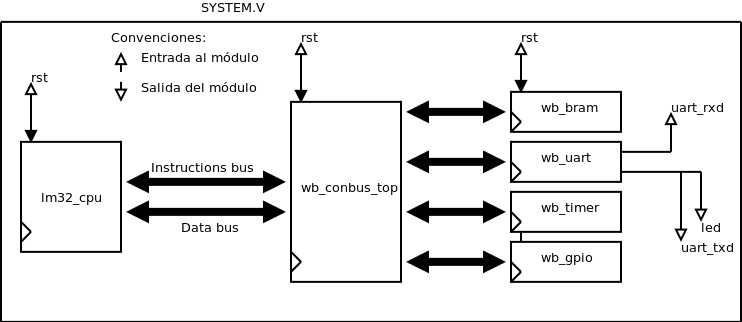
\includegraphics[scale=0.4]{system_v.png}
	\caption{Diagrama Simplificado para el \textit{System.v}.}
	\label{fig1}
\end{figure}


\section{Conclusiones}
\begin{itemize}
 \item Las herramientas de instalación proporcionadas al principio del curso fueron de gran ayuda, lámentablemente las mismas desaparecieron durante el desarrollo de esta práctica. De tal modo que dificultó enormemente su desarrollo y por ende la obtención de los resultados esperados.
 \item El LM32 ofrece una gran versatilidad para el proceso de implemetación, ya que una de sus grandes ventajas es la programación en \textit{C}. El problema radica en el proceso de compilación y lograr obtener el aschivo \textbf{.S} y \textbf{.bit} para quemar la FPGA.
 \item .
 \item .
\end{itemize}

\bibliographystyle{ieeetran}
\begin{thebibliography}{99}
\bibitem{patterson} Patterson, David \& Hennessy John
{\em "`Computer Organization And Design - The Hardware-Software Interface"'}.
Kindle Edition, Fourth Edition, 2006.

\bibitem{page1} \url{http://www.latticesemi.com/products/intellectualproperty/ipcores/mico32/index.cfm}

\bibitem{page1} \url{http://www.ohwr.org/documents/68}

\bibitem{page1} \url{http://www.linuxencaja.net/wiki/Arquitectura_LM32_JPRR_%28261744%29}
\end{thebibliography}
\begin{landscape}
\begin{figure}[H]
	\centering
		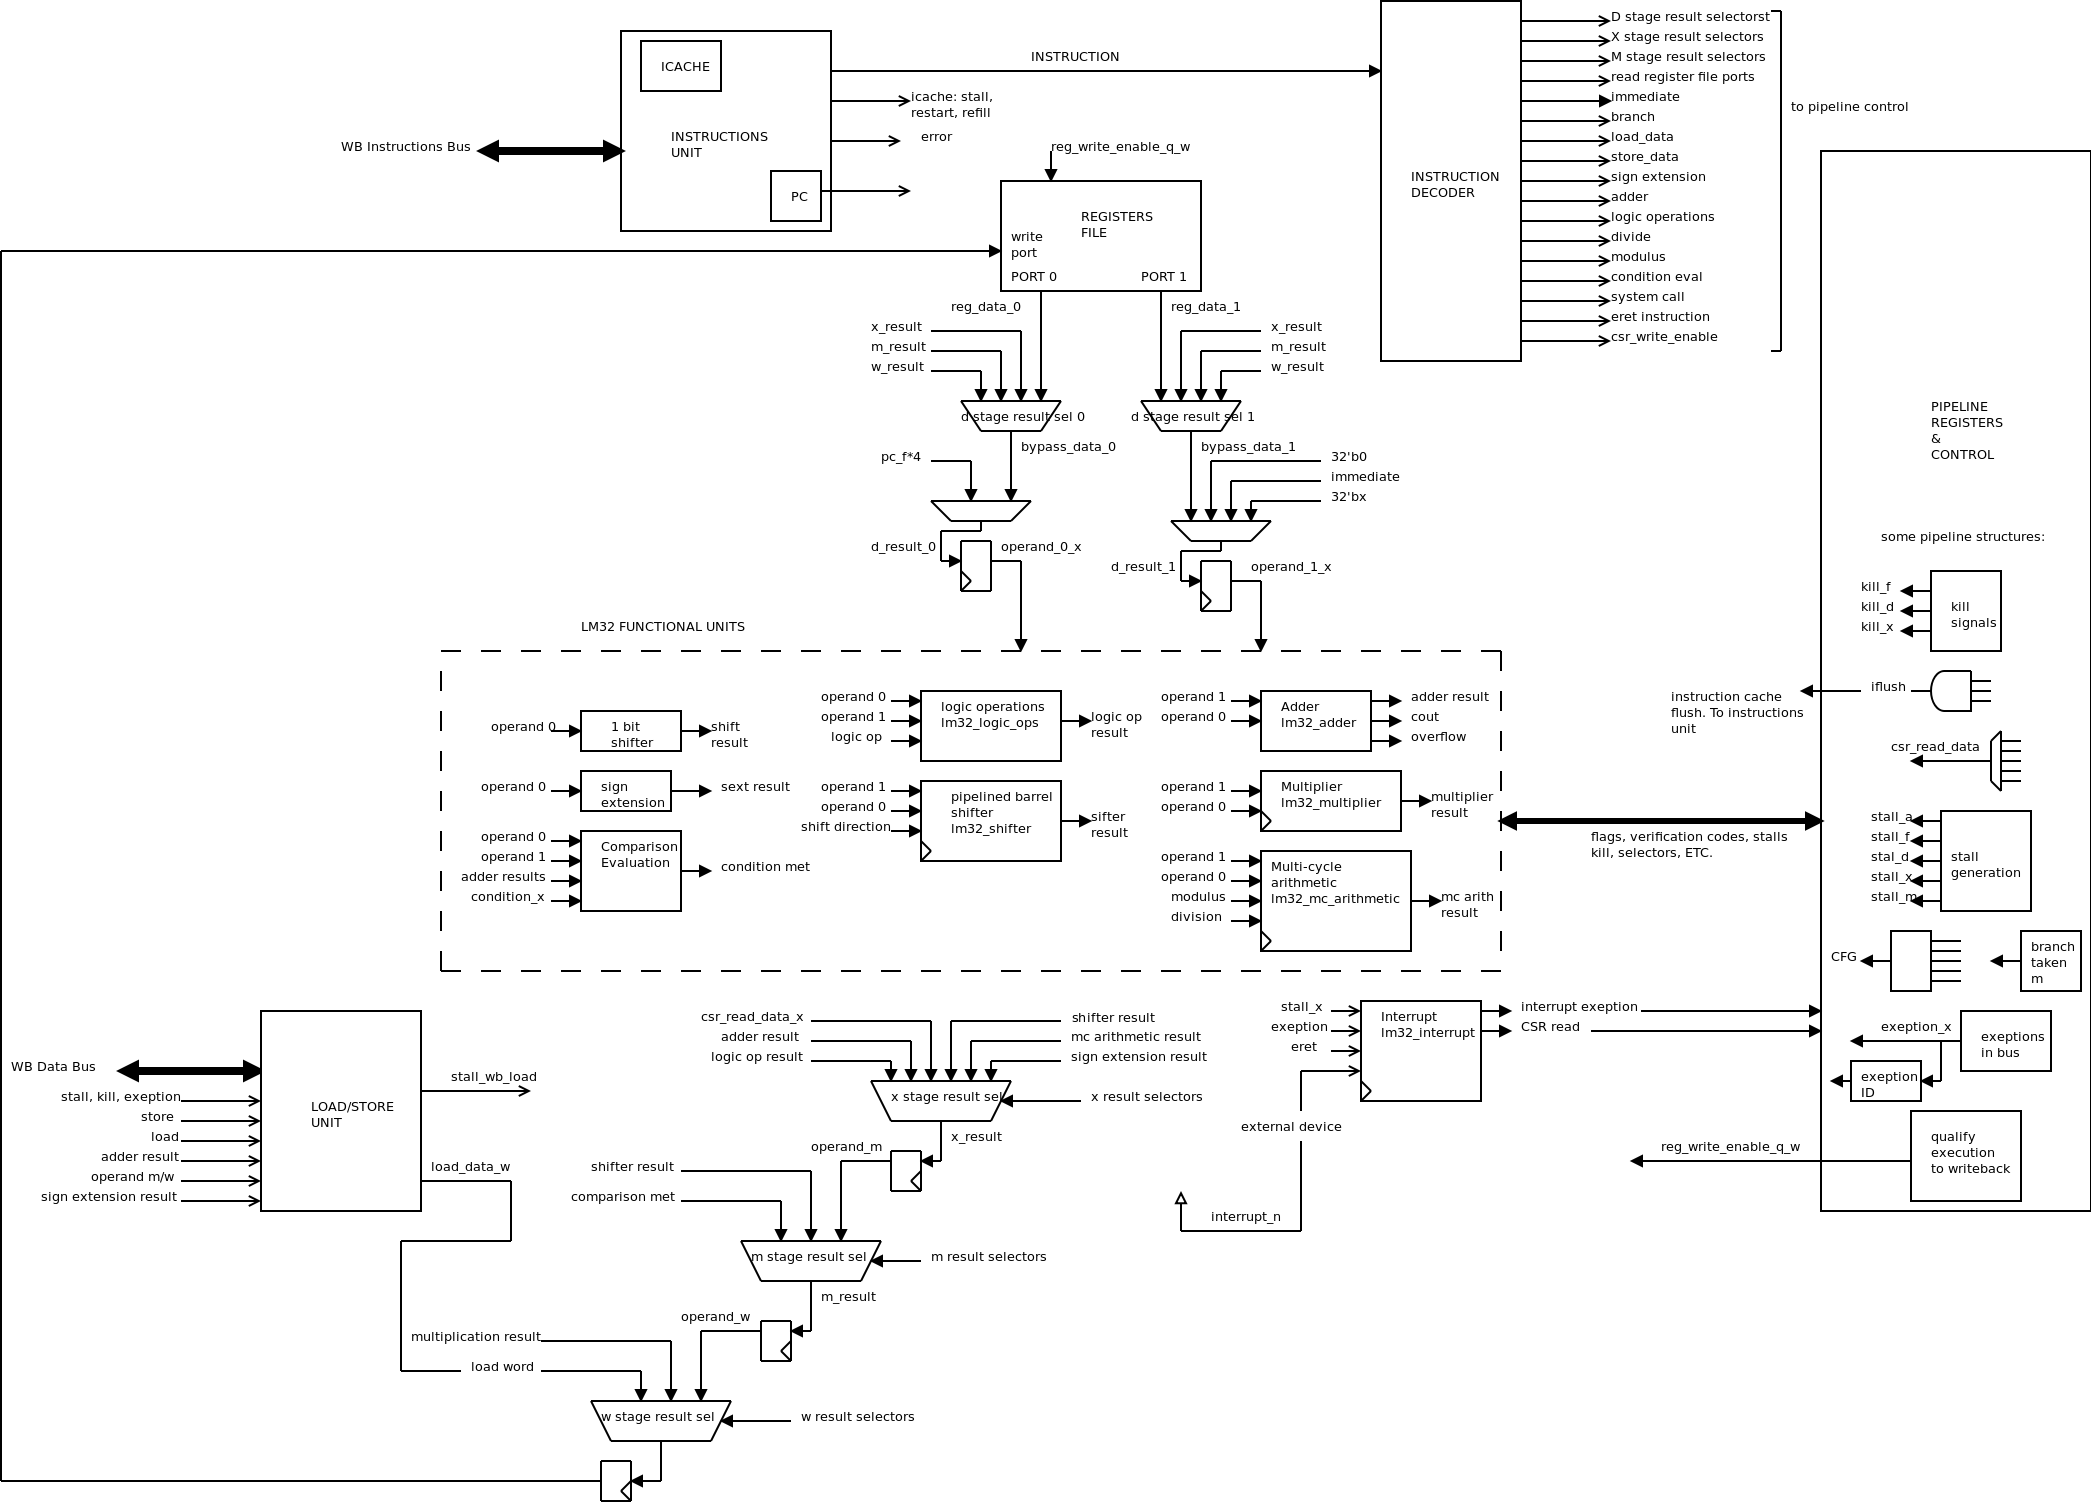
\includegraphics[scale=0.32]{DATAPATH.png}
	\caption{Diagrama completo para el \textit{datapath}.}
	\label{fig2}
\end{figure}
\end{landscape}
\begin{landscape}
\begin{figure}[H]
	\centering
		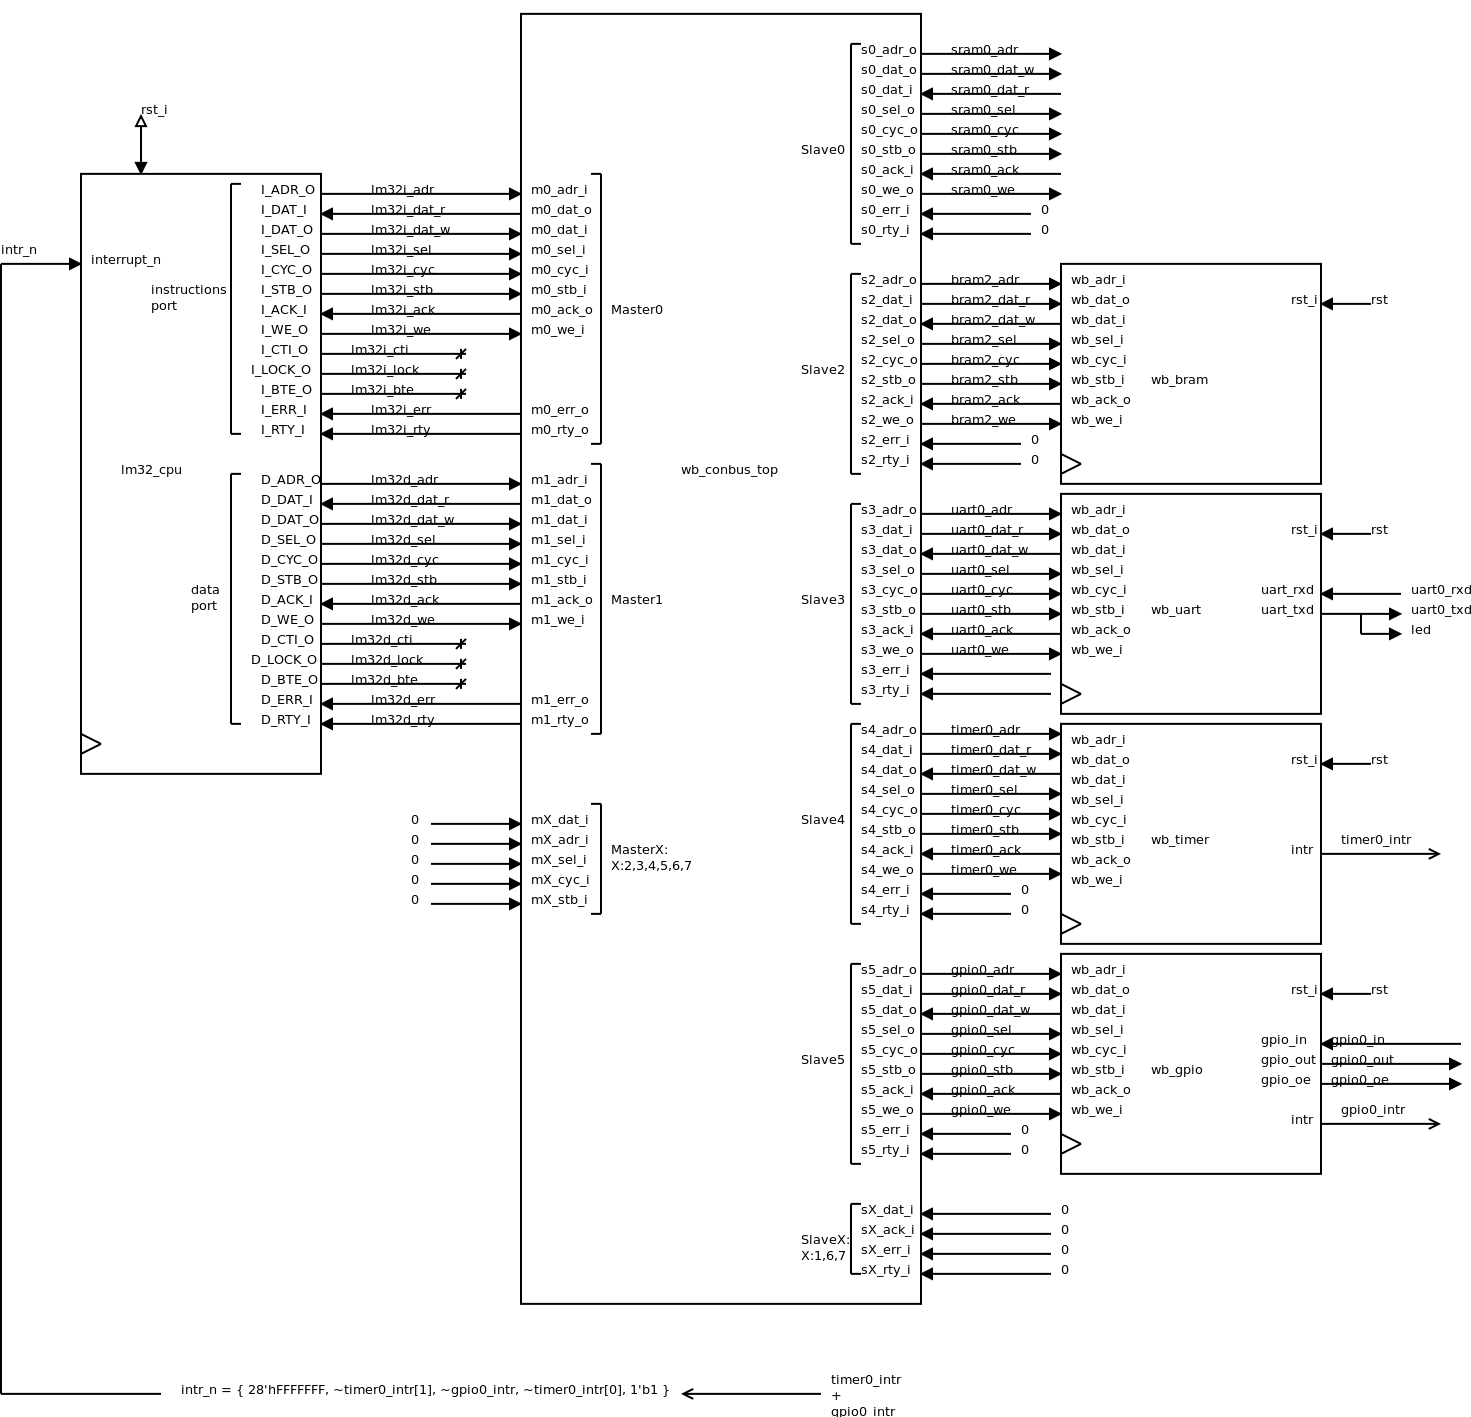
\includegraphics[scale=0.34]{system_v2.png}
	\caption{Diagrama completo para el \textit{System.v}.}
	\label{fig3}
\end{figure}
\end{landscape}
\end{document}